\chapter{Sortierverfahren}

\section{Lösung}

\begin{itemize}
    \item Es gilt, dass jedes allgemeine Sortierverfahren mindestens $\Omega(n\ log\ n)$ Schlüsselvergleiche benötigt (vgl.~\cite[154]{OW17b}).\\
    Diese untere Schranke gilt sowohl für die \textit{elementaren Sortierverfahren}\footnote{s. ~\cite[81]{OW17b}}  (\textbf{Insertion}-,
    \textbf{Selection}- und \textbf{Bubble}-Sort), die im \textbf{worst-case} $O(n^2)$ Zeit benötigen, als auch für die
    Verfahren, die eine \textbf{divide and conquer}-Strategie implementieren, wie \textbf{Quicksort} ($O(n^2)$)
    und \textbf{Merge-Sort} ($O(n\ log\ n)$ ).

    \item Bei sehr wenigen Datensätzen (in der Aufgabe mit $n \leq 100$ angegeben) ist die Wahl des Sortierverfahren
    hinsichtlich Effizienz im Sinne von Speicherplatzverbrauch als auch der benötigten Laufzeit eher nebensächlich, wenn man davon ausgeht,
    dass das Sortieren auf einem der heutigen Technik entsprechenden Rechner mit einem der o.a. Verfahren durchgeführt wird.\\
    Qualitätskriterien wie Einfachheit der Implementierung und Verständlichkeit können hier eher ins Gewicht gefallen (vgl. \cite[5 f.]{GD18a}).

    \item Andere Kriterien, die die Eingabedaten betreffen, können jedoch die Auswahl des Sortierverfahrens beeinflussen: Sind die Daten überwiegend
    vorsortiert, kann bspw. \textbf{Insertion-Sort} verwendet werden, das bei vorsortierten Daten lineare Laufzeit erreichen kann (vgl. \cite[188]{CL22})\footnote{
        \textit{Ottmann und Widmayer} führen außerdem \textbf{Smoothsort} von Dijkstra an, dass $O(n)$ für eine vorsortierte Folge und $O(n\ log\ n)$ benötigt (vgl.~\cite[112]{OW17b})
        }.

    \item Bei kleinen Problemgrößen fällt genau die damit verbundene Anzahl der Eingabedaten $n$ stärker ins Gewicht.
    Benötigt bspw. eine Implementierung von Insertion-Sort $8*n^2$ Schritte und eine Implementierung von Merge-Sort $64*n\ log\ n$ Schritte, so ist
    Insertion Sort für $n \leq 43$ effizienter als Merge-Sort (s. Abbildung~\ref{fig:insertionvsmerge})\footnote{
    \textit{Cormen et. al.} empfehlen einen \textit{Hybrid} aus Merge-Sort und Insertion-Sort in \cite[45, Problem 2-1]{CL22}, worauf auch \textit{Sedgewick und Wane} in \cite[275]{SW11} hinweisen.
    } \footnote{
        bei einem direkten Vergleich von Merge-Sort und Bubble-Sort dürfte schnell klar werden, dass ein unsortiertes Feld mit $n=2$ von Bubble-Sort mit weniger Operationen sortiert wird, als das bei Merge-Sort der Fall ist, wo neben dem Sortieren und Verschmelzen der Eingabefolgen außerdem zusätzlich linear viel Speicher für die Teilfolgen benötigt wird.
    }.

    \item In der Literatur finden sich Empfehlungen für Quick-Sort, das für typische Eingabedaten im Durchschnitt $O(n\ log\ n)$ Zeit benötigt und in-place arbeitet (vgl. \cite[182 ff.]{CL22}).

    \item Für eine hohe Zahl von Datensätzen, die auch im \textbf{worst-case} optimale Laufzeit aufweist, kann \etxtbf{Merge-Sort} verwendet werden, das mit $O(n\ log\ n)$ \textit{worst-case-optimal} ist (vgl.\cite[116]{OW17b}).
\end{itemize}


\begin{figure}
    \begin{center}
        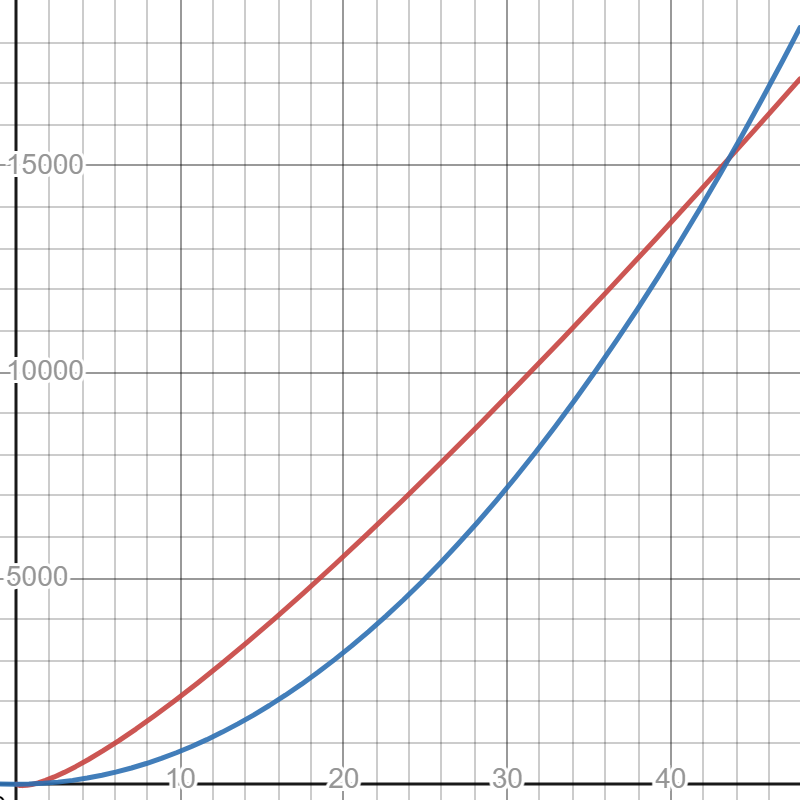
\includegraphics[scale=0.3]{chapters/7. Sortierverfahren/img/insertionvsmerge}
        \caption{Für eine Eingabelänge von $n\leq43$ arbeitet eine Implementierung von Insertion-Sort, die im Beispiel $8*n^2$ Schritte (blau) benötigt, effizienter als eine Implementierung von Merge-Sort, die im Beispiel $64*n*log\ n$ Schritte (rot) benötigt. (Quelle: eigene)}
        \label{fig:insertionvsmerge}
    \end{center}
\end{figure}